Despite there is already a discussion regarding every single use case, it is always important to create a general overview of discussion over the research, discarding specific projects or implementations. With this in mind there will be a discussion pointing out what were the results obtained through this research, a \textbf{SWOT} analysis for referring it's major aspects in a more abstract way and which research questions were answered and how they got answered. 
A general discussion is important, otherwise only the use cases will be considered and not the full extension of actually having the ideas of both conjured to a more general conclusion, focusing in general perspectives but also in the existent linkage between all of the factors and what is actually under research.

\paragraph{Putting all together}\mbox{}\\
In respect to what has been covered so far, within the discussion realm, it was noticed that for the first use case discussion was not that specific. This is because results were not taken into account due to the fact that it was more theorical-oriented, which means that no results were dragged to compare and delve into. However, since the second use case's a base for the theoretical scheme of the first use case, providing it's blockchain infrastructure to store file hash representations becomes feasible to test the overall idea. As such, future work about gathering both dimensions will be covered in the appropriated section, giving the necessary insights to discuss until each measure using both ideas can be beneficial where all the mentioned architectures can come to play, and even the management of an \textbf{IPFS} node can be something that could potentially be managed by the same tool as the one covered in the \textbf{kubernetes} architecture. Regarding this aspect, it should be known that until reaching that level of robustness, a lot of work remains to be done, and overcomplicating the existing infrastructure is not a requirement. Thinking forward to see if such hypotheses are useful, minimal insights could be taken into account in case the previous tasks take too long, but that's something that should have its own place and time to succeed. Additionally, a lot more ideas and intriguing questions may surge, which makes this work even more interesting due to the fact that multiple probable scenarios may occur.

\paragraph{SWOT analysis}\mbox{}\\
In the following figure, a \textbf{SWOT} analysis will be conducted having both use cases combined. At this stage, this analysis will be done in a more general way. However, for covering in more depth aspects presented here, the suggestion remains to go to the before-mentioned use cases and see more concrete aspects that otherwise will be covered here at a more high level:

\begin{figure}[H]
	\centering
	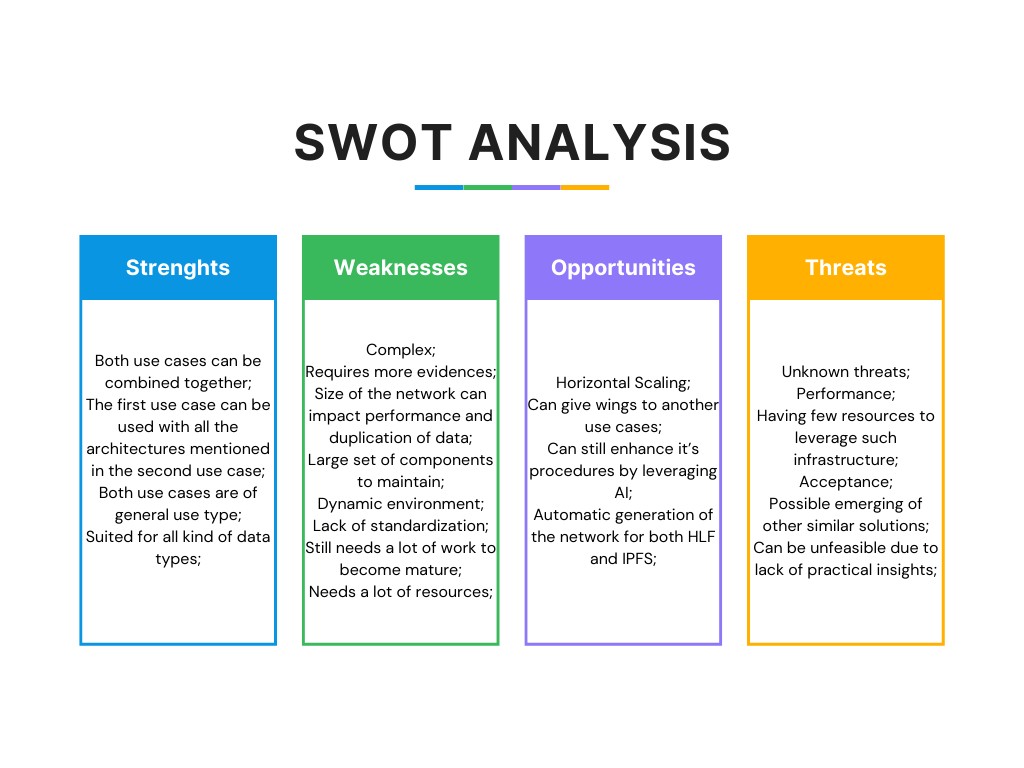
\includegraphics[width=0.9\linewidth]{assets/discussion/SWOT-analysis-general}
	\caption{Discussion: SWOT analysis}
	\label{fig:swot-analysis-general}
\end{figure}


\paragraph{Research Questions}\mbox{}\\
Coming across answering how the research questions "How can a private blockchain network be utilized to improve data integrity, security, flexibility, and collaboration within the healthcare ecosystem?" and "What kind of infrastructure design is necessary to support a blockchain solution in such a vast and complex environment as healthcare?" were answered, it should be known that the first one got answered in the state of the art, covering all the major aspects of the blockchain,it its types,it its influence in the healthcare sector, benefits, implementation requirements, current implementation challenges and issues, and its implementations. The second answer, however, was answered in more depth in the second use case, presenting a solution that could be leveraged to both smaller and larger environments, focused more in an on-premise environment, specially designed for healthcare environments, though not feasible in any use case.